\documentclass[]{article}
\usepackage[UTF8]{ctex}
\usepackage[a4paper,left=10mm,right=10mm,bottom=10mm,top=10mm]{geometry}
\usepackage{graphicx}
\usepackage{float}
\usepackage{amsmath,amsfonts,amssymb,amsthm}
%opening
\title{计算机科学中的数学基础 -- exercise W2}
\author{陈昱衡 521021910939}

\begin{document}

\maketitle
\section*{Homework9}
\begin{figure}[htb]
	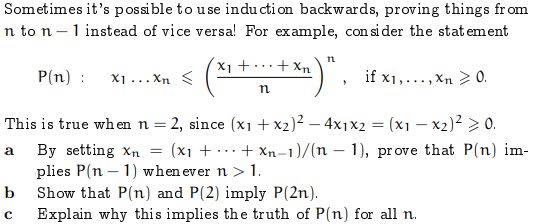
\includegraphics[scale=1]{Q9}
\end{figure}
\begin{enumerate}
	\item[(a)]
	If we want to prove P(n-1) using P(n),we can manage this by proving the following equation :\par 
	\begin{equation}
		x_{1}\cdots x_{n-1} (\frac{x_{1}+\cdots x_{n-1}}{n-1}) \le (\frac{x_{1}+\cdots x_{n-1}}{n-1})^{n}
	\end{equation}
	It's quite easy,as we can use the inequality:\par 
	\begin{equation}
		(\frac{x_{1}+\cdots x_{n-1}}{n-1})^{n-1} \ge (\frac{x_{1}+\cdots x_{n}}{n})^{n}
	\end{equation}
	\item[(b)]
	From P[n],we can get:\par
	\begin{equation}
		x_{1}\cdots x_{n}x_{n+1}\cdots x_{2n} \le ((\frac{x_{1}+\cdots+ x_{n}}{n})(\frac{x_{n+1}+\cdots+ x_{2n}}{n}))^{n}
	\end{equation}
	then using P(2),we can further get :
	\begin{equation}
		((\frac{x_{1}+\cdots+ x_{n}}{n})(\frac{x_{n+1}+\cdots+ x_{2n}}{n}))^{n}
		\le
		(\frac{x_{1}+\cdots+ x_{2n}}{2n})^{2}
	\end{equation}
	then the question got proved.\par 
	\item[(c)]
	Using the conclusion we got from (b),since we got P(2) now,then we can got P(4),using (a),we can get P(3).So,we can keep getting P($2^{k}$) using (b),and get P($2^{k-1}+1$) to P($2^{k}-1$).
\end{enumerate}

\section*{Homework11}
\begin{figure}[H]
	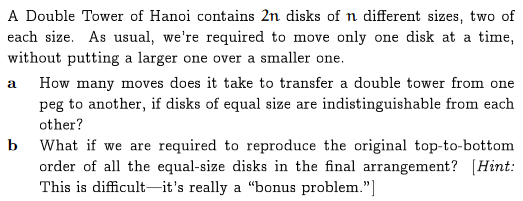
\includegraphics[scale=1]{H11}
\end{figure}
\begin{enumerate}
	\item[a] 仿照经典汉诺塔问题的思路,由于最下面的两个盘子是等大小的,所以可以一起处理,即,每次处理两个相同大小的盘子。所以,过程就是:现将除去最下面两个盘子的其余盘子移到中间柱上,然后用2步移动最大的两个盘子到目标柱上。因此,可以得到递归式:
	\begin{equation}
		T_{2n} = 2*T_{2n-2} + 2 \quad (n \ge 2) \\
		T_{2n} = 2 \quad (n = 1)
	\end{equation}
	然后使用递归树,或者书中经典解法对递归式进行求解,可以得到:
	\begin{equation}
		T_{2n} = 2^{n+1} - 2
	\end{equation}
	\item[b] 易知,对于(a)中的过程,进行两次和(a)中过程一样的移动,得到的盘子和原先顺序一致。\par 
	因此,最少步骤的移动方式为:
%	先用$T_{2n-2}$步将上面2n-2个盘子移动到C,再将
\begin{figure}[H]
	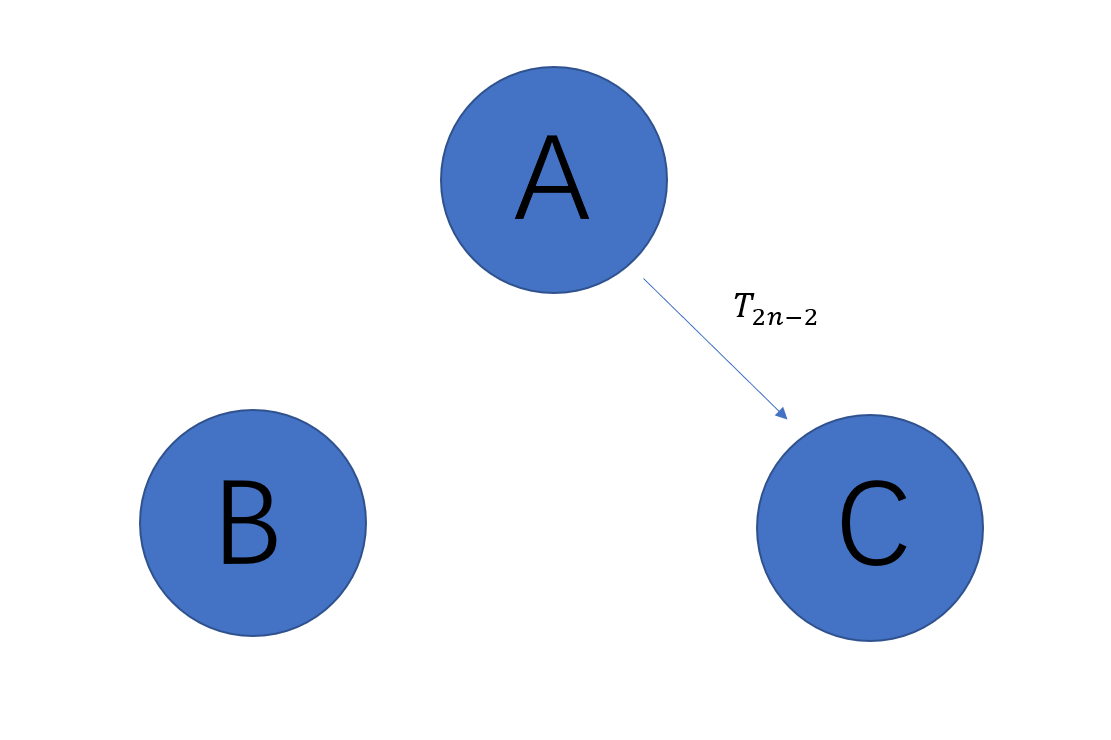
\includegraphics[scale=0.4]{P1}
	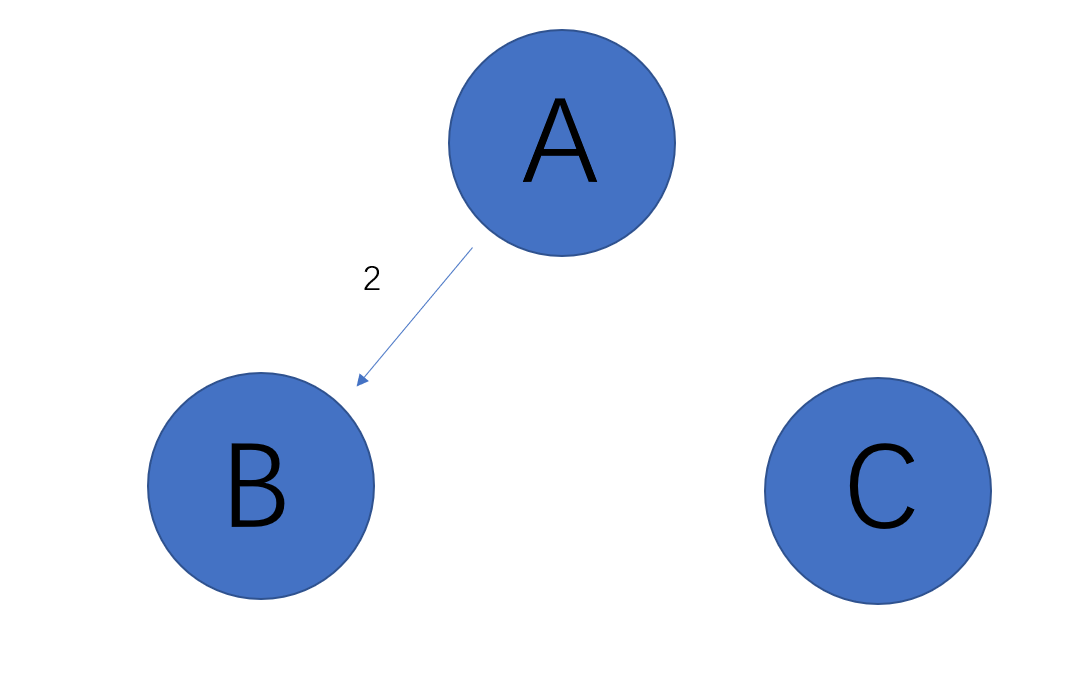
\includegraphics[scale=0.4]{P2}
	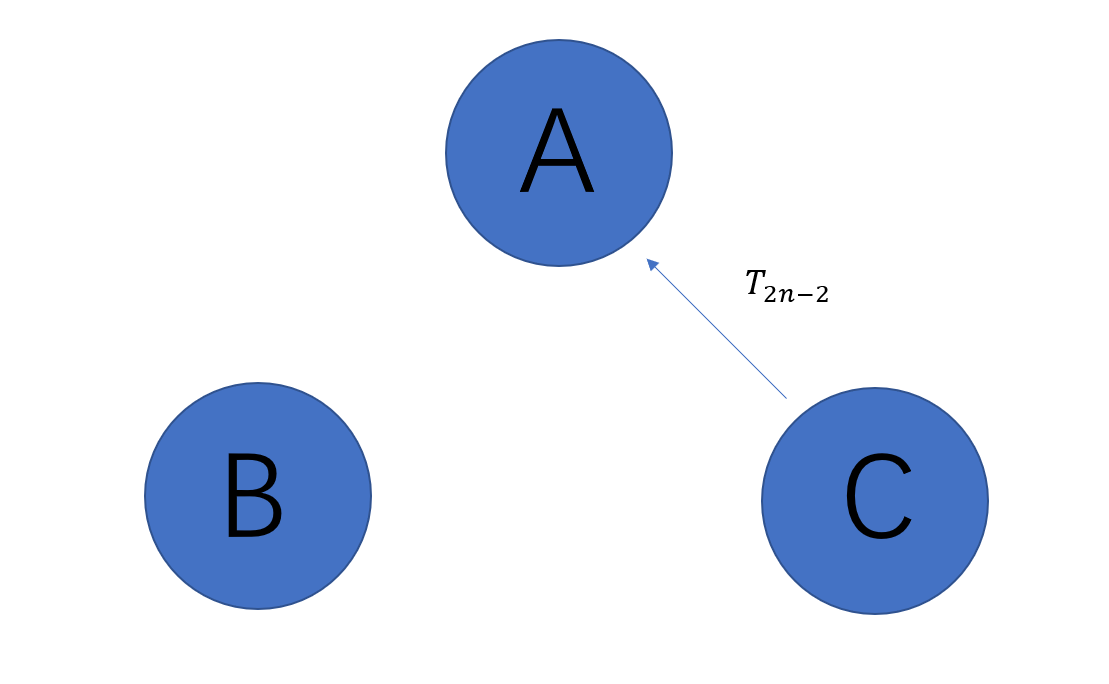
\includegraphics[scale=0.4]{P3}
	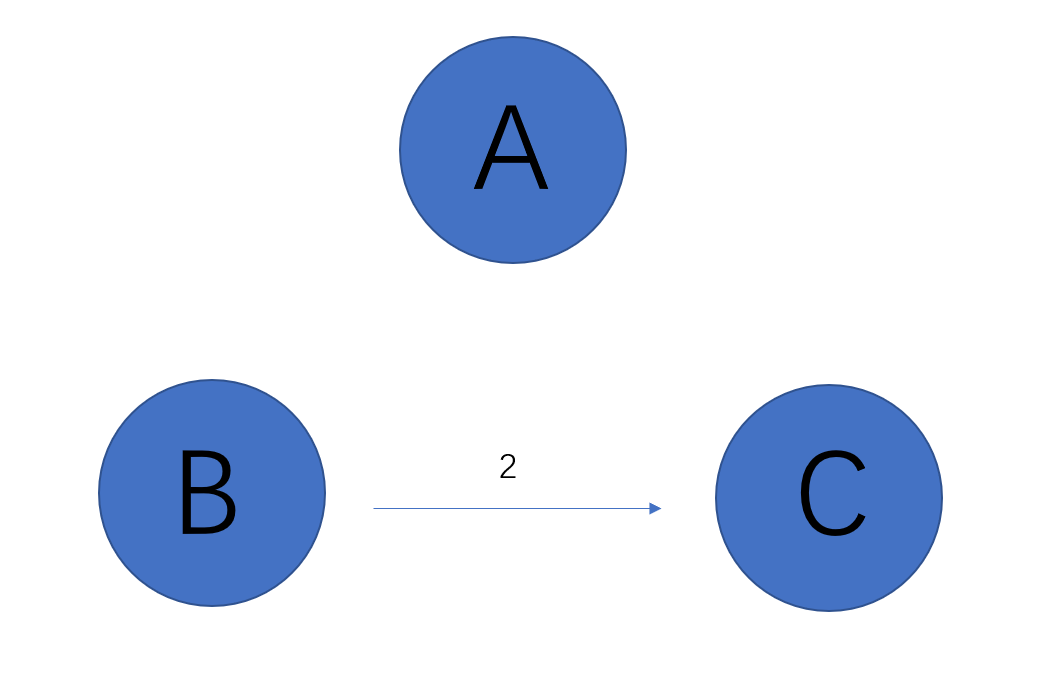
\includegraphics[scale=0.4]{P4}
	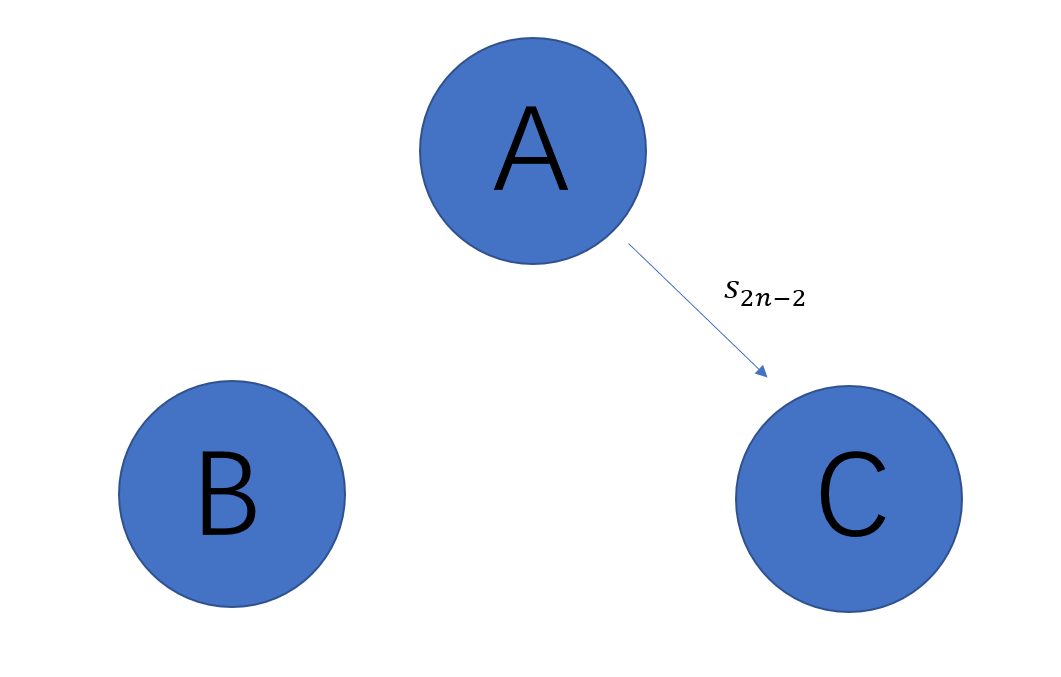
\includegraphics[scale=0.4]{P5}
\end{figure}
由此,我们可以得到递归式:
\begin{equation}
	S_{2n} = 2 * T_{2n-2} + 4 + S_{2n-2}
\end{equation}
求解得,
\begin{equation}
	S_{2n} = 2^{n+2}-5
\end{equation}

\end{enumerate}


\section*{Warmup1}
\begin{figure}[htb]
	\includegraphics[scale=1]{W1}
\end{figure}

由本章第一节中对记号的定义,原式表达的含义是从k=4到k=0之间的$a_{k}$累加。而$4 \le k \le 0$中包含0个符合条件的k,故原式为0。


\section*{Warmup2}
\begin{figure}[htb]
	\includegraphics[scale=1]{W2}
\end{figure}


题干中[x > 0]的含义为:\par 
\begin{equation}
	x = \left\{ \begin{array}{rl} 0 & 
		\text{if } x <= 0,\\ 1 & \text{if } x > 0. \end{array} \right.
\end{equation}
[x < 0]类似。\par 
因此,原式的含义为$|x|$.\par 

\section*{Warmup3}
\begin{figure}[htb]
	\includegraphics[scale=1]{W3}
\end{figure}
由课本中关于求和符号的定义:我们将 
\begin{equation}
	\sum_{P(k)} a_{k}
\end{equation}


记为所有项  $a_{k}$之和的缩写,其中的 k 是满足给定性质 P(k) 的一个整数.\par 
因此,由不等式$ 0 \le k \le 5 $ 解出k=0,1,2,3,4,5,因此
\begin{equation}
	\sum_{0 \le k \le 5} a_{k} = a_{0} + a_{1} + a_{2} + a_{3} + a_{4} +a_{5}  
\end{equation}

同理,由不等式$ 0 \le k^2 \le 5 $ 解出k=0,-1,1,-2,2,因此
\begin{equation}
	\sum_{0 \le k \le 5} a_{k} = a_{0} + a_{1} + a_{1} + a_{2} + a_{2}  
\end{equation}

\section*{Warmup4}
\begin{figure}[htb]
	\includegraphics[scale=1]{W4}
\end{figure}
\begin{enumerate}
	\item[a] 可以首先求出i,j,k的范围,分别是$1 \le i \le 2,2 \le j \le 3,3 \le k \le 4$,所以可以写出:
	\begin{equation}
		\sum_{1 \le i \le 2}\sum_{i+1 \le j \le 3}\sum_{j+1 \le k \le 4}a_{ijk} = ((a_{123}+a_{124})+a_{134})+a_{234}
	\end{equation}

	\item[b] 由(a)中i,j,k的范围,再结合求和的顺序,可以写出:
	\begin{equation}
		\sum_{3 \le k \le 4}\sum_{2 \le j \le k-1}\sum_{1 \le i \le j-1}a_{ijk} = ((a_{134}+a_{234})+a_{124})+a_{123}
	\end{equation}
\end{enumerate}

\section*{Warmup5}
\begin{figure}[htb]
	\includegraphics[scale=1]{W5}
\end{figure}
虽然j和k的取值范围相同,但是j和k是不同的指标,$a_{j}$和$a_{k}$也未必是相同值。使用统一的指标k去替代两个独立的,不相同的指标显然是错误的。\par 
尽管当 $a_{k} = a_{j} (1 \le k \le n,1 \le j \le n)$,结果是正确的,但是推导过程依然是错误的。\par 




\end{document}
